\chapter{Analytics Tools used in this research}
\label{appendix-analytics-tools}

This chapter complements the `On Mobile Analytics` chapter. That chapter covers the key elements and concepts, this one describes the analytics tools we used during my research.


\section{Classifications of Mobile Analytics tools}~\label{classifications-of-mobile-analytics-tools-used-in-this-research}
The case studies also facilitated the study of various mobile analytics tools. A map of these tools and the case studies they were used in may help the reader (and the author). Here are suggested topics to consider for each of these tools.
\begin{itemize}
    \itemsep0em
    \item To consider: which projects was the tool used in/relevant to?
    \item What was the tool used for?
    \item What insights did we glean from using the tool?
    \item If anythings made the tool distinctive, what were those things and why are they distinctive in the context of developers using mobile analytics?
    \item Type of the analytics and where in the application stack it collects the analytics.
    \item APIs and optional capabilities:
    \begin{itemize}
        \item Application APIs: that can used in the app to customise what is sent
        \item Reporting APIs: that can be used to obtain the data and reports, etc. 
    \end{itemize}
    \item Customisation of reporting, if any.
    \item Data output options (see the appendix on Data Sources for the current known set of output options).
    \item Platform(s) supported.
    \item Some notes on data retention facilities and limitations.
\end{itemize}
\textbf{Vitally} how the tool(s) were used in each case study. Worry less about the complete capabilities of these tools, especially as some are now defunct and no longer available or viable in terms of future research.

\subsection{Mobile Analytics tools used in this research}
\begin{itemize}
    \item Android Vitals (integrated into Google Play Console)
    \item AppPulse Mobile (when owned by HP)
    \item Azetone heat mapping together with some collaboration with Appsee
    \item count.ly
    \item Crashlytics (when owned by Google and branded as Fabric, and briefly after it was migrated to Firebase)
    \item Flight Recorder (now defunct)
    \item Sentry
    \item Iteratively
    \item Microsoft App Center
    \item Google Firebase Analytics
    \item Google Play Console (2018-2020 and 2020-2021 editions)
\end{itemize}


%%%%%%%%%%%%%%%%%%%%%%%% AppPulseMobile %%%%%%%%%%%%%%%%%%%%%%%%%%%%%%%%
\section{AppPulse Mobile}

Open API \href{https://github.com/MicroFocus/apmobile-openapiclient/blob/master/doc/AppPulse_Mobile_Open_API_Guide.pdf}{Open API Guide} and a  \href{https://github.com/MicroFocus/apmobile-openapiclient}{sample client for AppPulse Mobile's Open API}

``Open API – Resource Usage: Extract battery usage and cellular usage data to create custom reports integrated with external systems and dashboards. New APIs help you mine resource usage metrics from your user’s devices and operating systems." from ``What's New in AppPulse Summer '16 Release"

\begin{itemize}
    \item ``...tested an hybrid application, this requires to turn a special flag in the instrumentation process, I assume it wasn’t turned on and that is the reason for not capturing some of the things." However: the \texttt{-hybrid} instrumentation flag which doesn't actually seem to exist in 1.96, perhaps it's only in a pre-release version
    \item ``AppPulse mobile requires internet access from the mobile device. We monitor the user actions, crashes etc. and report the statistics back to HP SaaS servers – sending the data is done over the internet."
    \item HP have made improvements to AppPulse Mobile as a result of working with me, so their library now captures more of the user actions (Sept 2015).
\end{itemize}

Findings: 
\begin{enumerate}
    \item How well does the client library cope in terms of storing and subsequently forwarding events, messages, whatever, in the following circumstances?
    \begin{enumerate}
        \item Use of a proxy server?
        \item When connected to a Wi-Fi that doesn't have internet access e.g. a local internal hotspot?
        \item When the network is unavailable e.g. when the device is in 'flight mode' without Wi-Fi or mobile network access?
    \end{enumerate}
    \item I saw an example where my app crashed on an Android 2.3 device (and old Google Nexus One) where AppPulse Mobile didn't record the crash.
    \item The FunDex score varied more than I expected, and sometimes changed as I navigated around the various sections of the UI. A pattern seemed to start to emerge but I didn't test it sufficiently to describe it accurately.
    \item Some UI events, and other events, don't seem to be captured by AppPulse Mobile. Examples include:
    \begin{enumerate}
        \item Read aloud text on the screen (triggered from a menu option)
        \item Navigation in a WebView
        \item Changing ease of access settings and other UI preferences
    \end{enumerate}
\end{enumerate}

I'd also appreciate knowing more about the data transmission aspect, such as message sizes, frequency of sending, whether it aggregates several events into a single transmission, etc.

BTW: I wonder how much it's been used with apps that support multiple UI languages (Kiwix for Android supports 100+). The screen labels are sometimes derived from the display language so they seem to be treated as separate elements in the user flows.]

Results:
\begin{itemize}
    \item The development team of the Analytics tool observed: ``I instrumented the apk, in general the instrumentation works. I do see some gaps, some missing actions, it’s because the application loads the content from the local file system - it seems that sometimes we don’t inject the instrumentation fast enough. I investigating it now and will let you know about the progress. [The] -hybrid flag is used in the java code internally, the shell script just passes the parameters." % Email source: https://mail.google.com/mail/u/0/#search/apppulse+mobile/FMfcgxmMlGKpJrtjFNcbGDcwpvBHHBjv
    \item [I discovered] AppPulse Mobile did not deliver events that occurred when the device had no internet connection. I proposed improvements to the AppPulse Mobile SDK so that it would store timestamped events locally and transmit them when the network connection was available. The improvements included considerations on the server-side processing of delayed events. %Original notes follow, the email source is: https://mail.google.com/mail/u/0/#search/apppulse+mobile/FMfcgxmNwpbfZkVPJpqFPrKMZjTjwxGW
    \item A bug in an analytics SDK didn't release memory for objects while scrolling a very long image list ( cart list) which caused the app to crash in production. An unanswered question was whether the built APK file was checked after the crashes occurred to determine whether optimisation practices such as zipalign were run correctly on it \url{https://developer.android.com/studio/command-line/zipalign.html} which reduces the memory footprint at runtime. Sources private correspondence with the SDK provider % https://mail.google.com/mail/u/0/#search/apppulse+mobile/FMfcgxmQHnbPSVLJShFHXvrxlccmzrJD
\end{itemize}

\begin{comment}
I've asked earlier to see if you could get AppPulse Mobile to be able to collect data (the analytics events) when there's no suitable network available, and where the data is safely recorded locally on the mobile device until such time as a viable network connection is available, then the data would be transmitted to the receiving AppPulse Mobile servers.

There are some design implications. Here are the main ones I consider:
Timestamping of event records. Perhaps the event records are already timestamped. If not, they, and their timestamps need to be transmitted, if we want to accurately process them.
Reporting of the data. As some data may arrive hours or even days after data that's been sent synchronously (from devices that had a working network connection), then reports may need to be recalculated and possibly retransmitted (and available as an update via the Open API's). There may need to be cutoffs in the system, possibly in the acceptance of 'old' data, possibly in the automated reports, possibly elsewhere.
How much data would be stored for how long on the local devices? FYI IIRC one of the similar genre of mobile analytics stores 5 discrete crashes while offline. Any more cause some data to be discarded. I don't know the details. It would be possible to calculate summary statistics and transmit those in cases where the AppPulse Mobile library has exceeded it's design/implementation/runtime storage limit(s). I'd hope the data could be stored for long periods and in relatively large volumes in terms of records. There are various techniques available to compress the data that's transmitted.
Having offline collection can help capture usage data and usage patterns that occur when the network is not available. In some cases the patterns may only happen when there's no viable network. For instance, apps may offer specific functionality when working in 'offline mode'.

Various competitors include support for offline data collection. My expectation is that as more people use AppPulse Mobile some will discover the lack of offline data collection and cause them to adversely consider the product as a result.
\end{comment}


%%%%%%%%%%%%%%%%%%%%%%%% HEAT-MAPPING %%%%%%%%%%%%%%%%%%%%%%%%%%%%%%%%
\section{Heatmapping: Azetone and Appsee}~\label{section-heatmapping}
Two heatmapping offerings were evaluated in 2015~\footnote{The date is particularly relevant as the industry has moved on significantly and one of these companies acquired in the interim.} partly in preparation for The Mobile Analytics Playbook~\citep{harty_aymer_playbook_2016} and partly to learn more about their capabilities in terms of providing mobile analytics. The two offerings were Azetone, provided by a French company, and Appsee, an Israeli company. %Confirmation https://techcrunch.com/2013/10/21/appsee/ 

The main focus of this case study was to determine characteristics of commercial heatmapping offerings for Android apps as a proof-of-concept for any further research. The evaluations were with the support and permission of the two companies who provided the offerings, they also provided additional materials about their products. 

There are various prerequisites to using the products:
\begin{enumerate}
    \item Obtain an account and the respective SDK key. Some providers offer either time-limited or a free tier that generally includes a subset of their overall service offering. 
    \item Integrate the relevant SDK and add the necessary call to the SDK passing in the SDK key as a parameter.
    \item Deploying the app with the integrated SDK and the app being used to generate the raw data that is then processed as part of the service.
    \item Observing the analytics provided online.
\end{enumerate}

If the analytics are to be calibrated then the usage needs to be known so the analytics and reports can be compared to the actual source activities.



\subsection{Azetone (in 2015)}
\begin{itemize}
    \item ``by default our SDKs are reporting back to the servers with a delay which can be up to 15 hours (to minimize bandwidth and resource consumption)"
    \item  \texttt{IntentReceiver com.immersion.android.haptics.HapticFeedbackManager\$HapticFeedbackBroadcastReceiver@41d4fe50} integrated into their Android SDK
    \item Record in admin mode ``make sure you use connect to your App in Admin mode to gather the different screens you want Heatmaps on…"
    \item Configuration options: optional call to increase the level of logging, explicit call to set the dispatch period to 240 seconds,
    \item Flaws in the reports: A system that's never been used should indicate it's never been used and is 'at-rest', whereas I've currently used (got) 20 users and even improvements on last month. application's name still appears as abcdef in the dashboard.
    \item  I decided to apply for a free trial of Azetone, however I discovered they a) don't make the Android SDK available, they only email (automatically) the iOS one, and b) they prohibit using with opensource softwware - so I've emailed their generic 'welcome' email address asking for permission to use their SDK with opensource apps, as I want to try it with Kiwix, etc.
    \item I've been trying to use Azetone's heatmap software / service. So far I've found numerous problems trying to get started, including various login problems, broken links, problems creating an app, naming an app, etc. I've yet to actually try integrarting their SDK, however I hope I'll now be able to finally do so.
    \item (mid Aug 2015) A quick update: I've made some progress with Azetone and first David (the CTO) then Philippe (who you know) introduced themselves after I'd sent them various feedback on the challenges I was facing and my observations of their platform. Philippe kindly explained they'd recently launched the self-service model (before the handheld their customers through the process). He also offered an extension until the end of November in return for my feedback and help. All good stuff. I decided to explain our relationship and that I know of his work, it seemed a good time to do so now I've got this far in the process. I've yet to see any results from using their heatmap SDK (I'm trying it with Kiwix again, as I did for AppPulse Mobile). I'll keep going until I/we either get it to work or they tell me it's broken.
    \item (27 Aug 2015) When I tried to create an application called kiwix-android I don't get an error message when I press 'create' or any other indication that anything's happened apart from the name I used diappears. When I then try to navigate elsewhere in the UI I'm taken to a login page. That login page doesn't accept my login with the correct password (one your site assigned after I used the 'forgot my password' service. However when I used the back button in my browser I was able to return to the dashboard UI. I eventually tried a simple, stupid application name of abcdef (IIRC) which was accepted and then displayed a fancy dashboard. Please can you improve your web site so:
    \begin{itemize}
        \item a) it allows more complex application names (I wanted to create kiwix-android and kiwix-ios, for instance)
        \item b) it tells the user if the name is not acceptable
        \item c) it does not force me to login again for no sane reason
        \item d) if it does, please at least let me login properly rather than having to use by browser's back button :)
    \end{itemize}
    \item (\nth{27} Aug 2015) Hmmm, do you have real users using this web site? I ask what seems like an insane question as I managed to get redirected to \texttt{'localhost'} i.e. a link intended to go to your internal computer, rather than your production web site. Here's the URL I was taken to: \url{http://localhost/azt\_dashboard/html/dashboard/res\_initialize.php} when I clicked the Resources link (see below for the raw text)  \url{https://dashboard.azetone.com/application.php} (the URL which contains the broken link)

\end{itemize}
Sources include email correspondence and my notes at the time.

\href{https://www.azetone.com/mobile-ux-analytics/}{Understand, Optimize and Personalize your UX - UX Analytics for iOS and Android}

\section{Examples of flaws in mobile analytics offerings}
\subsection{Azetone [Heatmaps]}
Some quirks in the system at rest and never been used: as the following extract, in Figure \ref{fig:azetone_dashboard_flaws_for_kiwix_2015}, of a screenshot shows - a brand new account has some quirks that don’t seem correct:
\begin{itemize}
    \item The app structure at 0 is 33\% higher than last month
    \item For app structure and profiles set-up there is a bar, but not for the other indicators, which have none.
    \item Spurious percentages: 59\%, 29\% and 12\%
    \item 20 of 50,000 [users] used
\end{itemize}

\begin{figure}[htbp!]
    \centering
    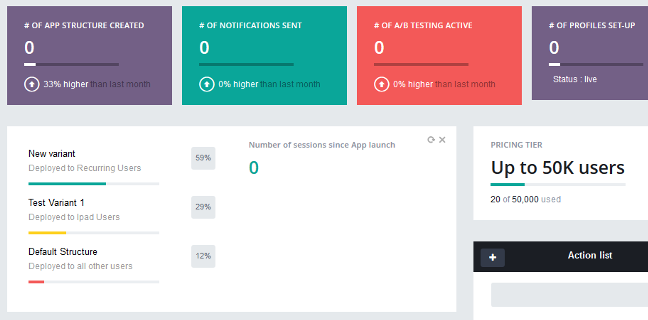
\includegraphics[width=12cm]{images/azetone/azetone_dashboard_flaws_for_kiwix_2015.png}
    \caption{Various flaws in Azetone's dashboard for a new project (2015)}
    \label{fig:azetone_dashboard_flaws_for_kiwix_2015}
\end{figure}

Comment from their CEO \emph{``FYI, by default our SDKs are reporting back to the servers with a delay which can be up to 15 hours (to minimize bandwidth and resource consumption)."}. However, during my limited evaluation no heatmaps appeared in their dashboard for our project.

\subsection{Appsee (in 2015)}
Individual recordings, aggregate heatmaps: Slide 4: ``Visualize both single user data (user replay) and aggregated user behaviour (touch heatmaps)" This point is insightful, and explains how both individual information and aggregate information are relevant and useful.

Slide 5: I like the comparison between "Gives the Why" and "Gives the What". However I think the quote favours themselves (as one might expect) and underplays how other mobile analytics can help. Also, from a privacy perspective, there's a general dislike and disquiet about such intrusive monitoring (visual monitoring, recording interactions, etc.) I sent you the spreadsheet with the results from my questionnaire on 17th, so app developers need to carefully consider whether visual analytics is worth the extra bandwidth usage and intrusion into users' privacy. 

\begin{figure}
    \centering
      \begin{minipage}[b]{0.4\textwidth}
        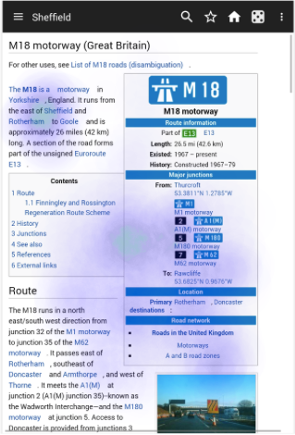
\includegraphics[width=\textwidth]{images/my/kiwix-appsee-slide.png}
        \caption{Slide gesture recorded by Appsee}
      \end{minipage}
      \hfill
      \begin{minipage}[b]{0.4\textwidth}
        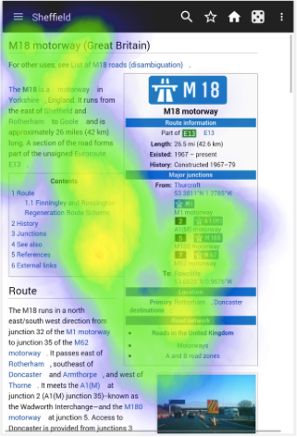
\includegraphics[width=\textwidth]{images/my/kiwix-appsee-zoom-dezoom.png}
        \caption{Zoom and Dezooms recorded by Appsee}
      \end{minipage}
    \caption*{Examples of Heatmapping using Appsee integrated into Kiwix Android}
    \label{fig:heatmapping-examples-kiwix-appsee}
\end{figure}
% Thanks to https://tex.stackexchange.com/questions/148438/putting-two-images-beside-each-other

Appsee far more polished than Azetone. For example, good first impressions of their terms of service and privacy agreements. It offered additional integration e.g. custom event messages, \href{https://web.archive.org/web/20150416132023/https://www.appsee.com/features/remote-configuration}{remote configuration}, \href{https://web.archive.org/web/20150317060748/https://www.appsee.com/features/crash-recordings}{recording of crashes and events that preceded the crashes}.

\begin{comment}
(From 2015)

While simple app analytics are great in providing numbers, they don’t reveal the full story. Appsee helps in understanding the reasons behind the numbers, while focusing on user behaviour. Appsee provides single session tracking, in addition to simple yet powerful reports based on aggregated data, and it's true power is the combination of the two. For example: you can see that 30\% of users quit the app from a certain screen, and then drill down to the single sessions to understand why.

In addition, Appsee provides visual analytics (such as heatmaps) - and automatically tracks all events in the app - so you don't have to think what to track, and makes sure that no interesting data is missed.~\href{https://web.archive.org/web/20150317073340/https://www.appsee.com/features/appsee-vs-analytics}{Appsee vs. Simple App Analytics}
\end{comment}

\href{https://youtu.be/GQ2DoINkba4?t=554}{Appsee-Optimizely Webinar: How to Perform the Ultimate A B Test with UX Analytics} %I've a copy of the slides sent by the then CEO Zahi

See also \url{https://www.youtube.com/watch?v=aRN\_XrxNCNE} %https://www.youtube.com/watch?v=aRN_XrxNCNE&spfreload=10


\url{https://medium.com/@Appseecom}



More information is available in \href{section-visual-gui-analytics}{section-visual-gui-analytics} on some early work pertaining to mobile app heatmaps. It also includes some recent updates on commercial heatmapping analytics.

%%%%%%%%%%%%%%%%%%%%%%%% Google Play Console w/Android Vitals %%%%%%%%%%%%%%%%%%%%%%%%%%%%%%%%
\section{Google Play Console incorporating Android Vitals}\label{google_play_console_section}

\subsection{Key Components of Google Play Console}
\subsubsection{Google Play Console UI}

TODO Describe each screen and the contents. Provide a table of the URL mapping and summary of their contents.

Name each graph and provide a screenshot so they can be discussed.

\begin{figure}[htbp!]
    \centering
    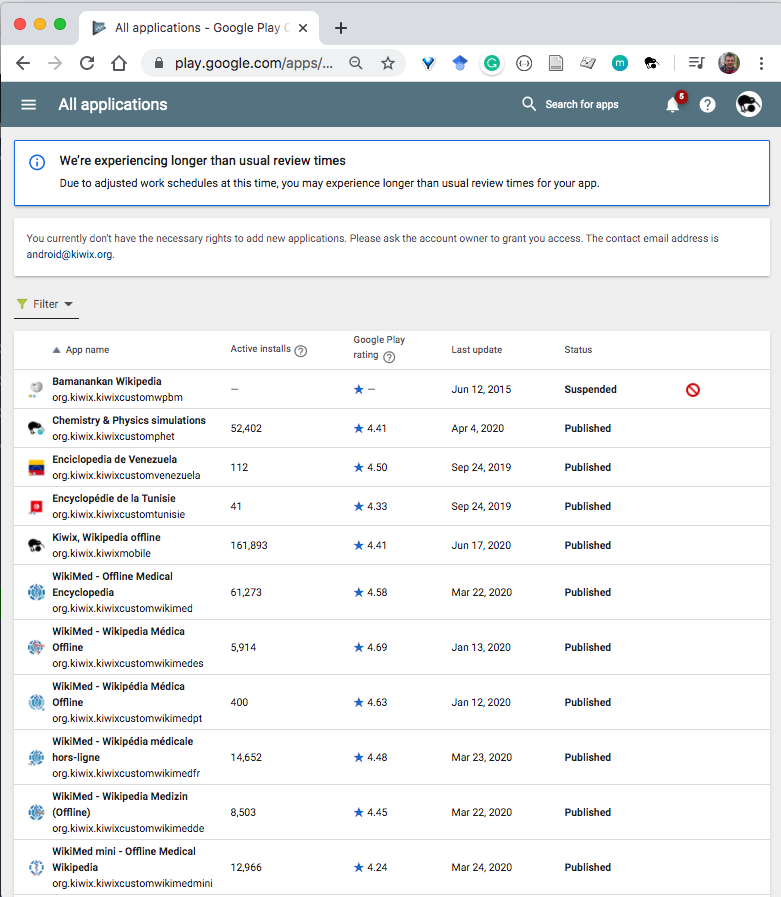
\includegraphics[width=15cm]{images/android-vitals-screenshots/AppListPlace-kiwix-2020-Jun-17.png}
    \caption{Google Play Console: AppListPlace for Kiwix project}
    \label{fig:gpc-applistplace-kiwix}
\end{figure}

\subsubsection{Release Management}
Mobile apps are released in the app store and there are defining events representing the start and end of each release. Releases take time to complete. During the release period the developers have some control on the rollout within the app store (they may also have controls within the app and/or in their related systems and services). Google Play Console provides them with the controls in the app store, it also provides three bands of reports, these are:

\begin{itemize}
    \item Release stability (which leads to Android Vitals)
    \item Ratings and reviews
    \item Installs and uninstalls
\end{itemize}

\begin{figure}
    \centering
    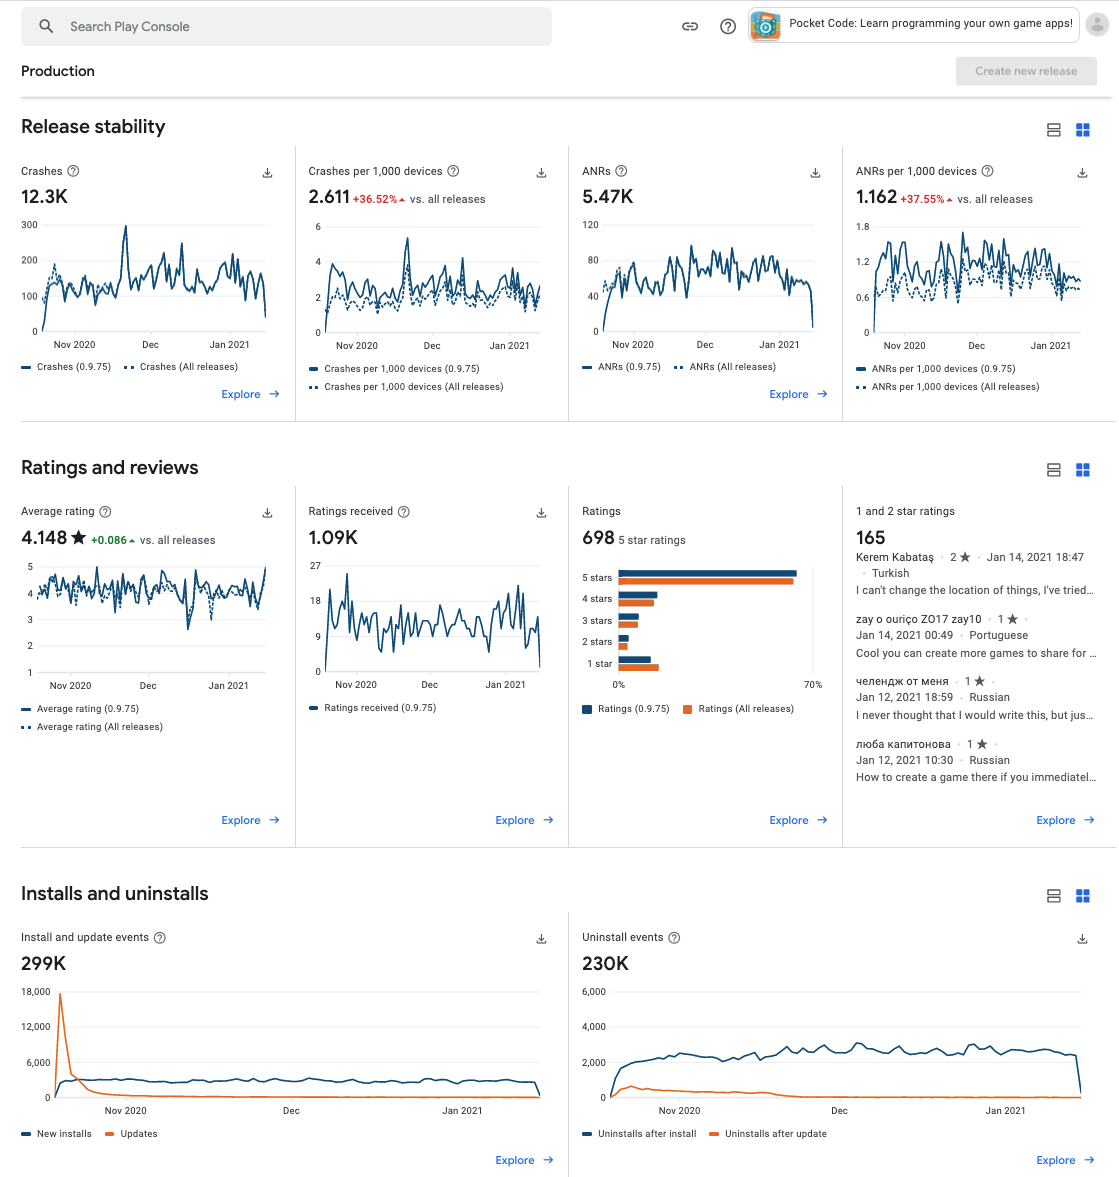
\includegraphics[width=12cm]{images/google-play-console/gpc-release-dashboard-pocketcode-v0.9.75-on2021-01-15.png}
    \caption{GPC: Release Dashboard for PocketCode V0.9.75}
    \label{fig:gpc-release-dashboard-pocketcode-v0.9.75}
\end{figure}

Figure~\ref{fig:gpc-release-dashboard-pocketcode-v0.9.75} provides an example of a recent release (0.9.75) of Pocket Code.


\subsubsection{Release Management: Release stability}


\subsubsection{Release Management: Ratings and Reviews}


\subsubsection{Release Management: Installs and uninstalls}




\subsection{Pre-launch reports}

~\url{https://stackoverflow.com/questions/48291106/security-warning-in-google-developer-console-pre-launch-reports-security-tab}

\subsection{Test channels}\label{subsection-test-channels}
MUST-DO complete this section.

\subsubsection{GPC Pre-launch Reports issues}
(December 2020)

\begin{itemize}
    \item \url{https://github.com/firebase/firebase-android-sdk/issues/2161}
    \item \url{https://stackoverflow.com/questions/64706041/fatal-exception-firebase-messaging-intent-handle-java-lang-noclassdeffounder}
    \item \url{https://issuetracker.google.com/issues/160907013}
    \item \url{https://forum.unity.com/threads/error-during-google-app-submission-java-lang-noclassdeffounderror-aewt.1005593/}    
\end{itemize}







\subsection{Android Vitals}
\subsubsection{Android Vitals UI}

\subsubsection{Peer Categories}~\label{section-peer-categories}
Peer categories may help developers to compare their app with various peer groups, those in the same category or sub-category as their app, and/or against a custom set of peers.

Android Vitals currently provides two distinct categories of comparative peer-based data: 1) predefined peers 2) a custom list of peers selected by the developer. The predefined peers are organised by category and sub-category. The categories match those available to developers when they list their app, there are 32 of them. There are 69 sub-categories (excluding the sub-categories that are All ... e.g. \texttt{All Education}). The sub-categories appear to be a subset of the 162 tags~\footnote{available on request, not essential for the thesis.} developers can use for their app store listing; for example \texttt{study guide} is both a tag and a sub-category, while \texttt{Prank} is only available as a tag. 

The full set of these 101 predefined peer categories with their respective sub-categories is shown in Table~\ref{tab:av-categories-with-crash-rates}~\footnote{Note: these were transcribed manually from the Android Vitals web UI and entered in a CSV file using Excel. The CSV file is read and processed when this thesis is compiled.}. This table shows the category and the median crash rate~\footnote{The ANR rates are also available for the same categories and sub-categories, they are not included currently, as they were not used in the research.} for that category.

The lowest crash rate, as measured by the median score is 0.18\% which applies to both \texttt{Productivity->Calendar} and \texttt{Productivity->Notebook}. The highest crash rate is 2.07\% for \texttt{Communications->Video Call}. Note: Google provide \textit{Personalization->Launcher} however the score is shown as \texttt{-}. % Todo calculate the variance.
 

There are some surprising and unexplained oddities in the data, for example \textit{Auto \& Vehicles->All Auto \& vehicles} has a median crash rate of 0.85\% and two additional sub-categories: \texttt{Auto \& Vehicles->Vehicle maintenance 0.73\%} and \texttt{Auto \& Vehicles->Vehicle shopping 0.27\%}. These are both significantly lower crash rates than the overall rate for this category - how can this be so? where are the data for the rest of the peer apps in this category presented? One possibility is perhaps they are collectively below a threshold to appear in either of the particular sub-categories?

The values are updated by Google on an ongoing basis and observations indicates they are updated once a day.

%%%%%%%%%%%%%%%%%%%%%%%%%%%%%%%%%%%%%%%%%
% Loading and displaying the CSV data took several hours to reach the following approach. I first tried using the csvsimple package however I came unstuck because the contents include characters latex interprets as formatting instructions. Also the data exceeds 1 page. I wasn't able to get multiple columns of the table working either, and trying to display the table landscape (to ensure there was enough linewidth to display several columns of the table didn't work either. 
% Thanks to various articles, in particular:
%   https://tex.stackexchange.com/a/269566/88466 from
%     https://tex.stackexchange.com/questions/269545/csvreader-and-respect-all-special-characters-in-the-csv-file
%   https://www.dickimaw-books.com/latex/admin/html/displaydb.shtml 
%   https://www.dickimaw-books.com/latex/admin/html/loadcsv.shtml
%  For csvsimple
%    https://stackoverflow.com/questions/62883114/latex-table-from-csv-file roughly the first thing I tried
%    https://tex.stackexchange.com/questions/358225/how-to-import-csv-table-with-header-containing-spaces was very useful, but the complexity of the file contents meant this failed to read in the content without errors.  I wish I'd seen https://tex.stackexchange.com/a/358226/88466 earlier as it introduced the alternative I ended up using.

%%%%%% This could do with a lot of polish e.g. to use a longtable which would allow me to reduce the space used. See p.127 in Latex for Administative Work Version 1.3 The raw sample code follows:
\begin{comment}
\begin{longtable}{cl}
\bfseries Country Code & \bfseries Country Name\\ \endhead \multicolumn{2}{r}{\emph{Continued on next page}} \endfoot \endlastfoot
\DTLforeach*{countries}{\Code=code,\Name=name}{\Code & \Name\\}%
\end{longtable}
\end{comment}

%%%% The current basic approach follows to list the Android Vitals categories.
\DTLloadrawdb[keys={a,b}]{t1g}{android_vitals_categories_with_crash_medians.csv}
{\footnotesize
\DTLdisplaylongdb
 [
   caption={Android Vitals Categories with median crash rates},% main caption
   contcaption={Android Vitals Categories (Continued)},% continuation caption
   % shortcaption={},
   label={tab:av-categories-with-crash-rates},% label
   foot={\emph{Continued on next page}},% table foot
   lastfoot={}% final table foot
 ]
 {t1g}
}

\subsubsection{Peer Groups in Android Vitals}\label{android-vitals-peer-groups}
% Google calls them peer groups.
Android Vitals offers developers the option to define a peer group of between 8 and 12 other apps in the Google Play Store. The peer group can be edited up to 3 times per month according to the documentation, and changes seem to take immediate effect in terms of the reporting~\footnote{\url{https://support.google.com/googleplay/android-developer/answer/9324048}}.

The daily crash rate for the peer group can vary which is interesting in terms of observing variations in their overall crash-rate; Figure \ref{fig:pocketcode_peer_crash_rate_18_nov_2019} illustrates the daily change for one of the case studies: the Pocket Code Android app. It is not likely to be easy to determine which of those apps spiked (as the list can only be updated 3 times per month, editing the list and observing the difference has a low likelihood of unmasking the peer, the author will leave designing approaches for future research).

\begin{figure}[htbp!]
    \centering
    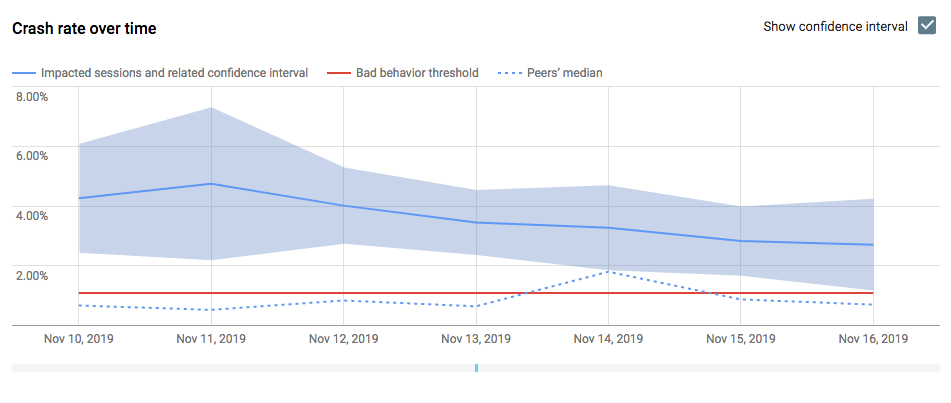
\includegraphics[width=\textwidth]{images/android-vitals-screenshots/peer-crash-rate-catrobat-18-nov-2019.jpg}
    \caption{Pocket Code peer crash-rate as of \nth{18} Nov 2019.}
    \label{fig:pocketcode_peer_crash_rate_18_nov_2019}
\end{figure}{}



\subsection{Monthly Report Files}

Google Play Console generates monthly reports, with the current month's report updated on a daily basis. 

%COULD_DO map screens or graphs to monthly report files.

\subsubsection{Access to the Monthly Report Files}
The reports are only made available for accounts which have 'global' read-only access\emph{`To access bulk reports, your "View app information" permission must be set to "Global."'}~\footnote{\url{https://support.google.com/googleplay/android-developer/answer/6135870\#export}}. Google explain why \emph{``Reports available on Google Cloud Storage use the same access restrictions that control data access on your Play Console. This means account users with access to areas of a Play Console account have access to the corresponding reports in Google Cloud Storage."}~\footnote{\url{https://support.google.com/googleplay/android-developer/answer/2528691}}  

\subsection{Google Play Console Revamp}
Google transitioned all users of Google Play Console from the previous version to a revamped version between June and 2nd November 2020. Developers were able to continue using the older version during the transition period by choosing the `classic' Play Console, this caused a URL parameter to be added~\texttt{\&noredirect} as demonstrated here
\url{https://play.google.com/apps/publish/?account=nnnnnnnnnnnnnn\&noredirect#AppListPlace} (the account number has been replaced to protect that account).

%%%%%%%%%%%%%%%%%%%%%%%% Fabric Crashlytics %%%%%%%%%%%%%%%%%%%%%%%%%%%%%%%%
\section{Fabric Crashlytics}

\begin{itemize}
    \item History of Crashlytics:
    \item Crashlytics, one of several products incorporated into Fabric.
    \item Migration of Fabric from Twitter to Google.
    \item Firebase eclipses and supersedes Fabric
\end{itemize}

\url{https://status.firebase.google.com/incident/Crashlytics/20001}

Google retired the Fabric products, including Fabric Crashlytics on \nth{4} May 2020. They provided a range of similar product offerings in Firebase. For Fabric Crashlytics they continue to support the Fabric Client API (presumably so developers did not need to modify their apps to continue collecting crash data) however the reports differ in the Firebase Console, and developers had to explicitly migrate their apps from Fabric to Firebase. The Catrobat development team experienced insurmountable issues trying to migrate all bar one of their Android apps that used Fabric Crashlytics. Seemingly a common flaw also prevents the project team from adding Crashlytics to new apps in their Firebase Account. The workaround the team used was to create a second unrelated account in Firebase and to use that account to configure Crashlytics for apps. %SHOULD-DO discuss the final migration process with Wolfgang and the Android and iOS development teams.


%%%%%%%%%%%%%%%%%%%%%%%% Firebase %%%%%%%%%%%%%%%%%%%%%%%%%%%%%%%%
\section{Firebase}
Firebase has come a long way from modest beginnings in 2011~\url{https://techcrunch.com/2012/04/19/firebase-post-launch/} and a change in focus~\url{https://techcrunch.com/2012/05/22/firebase-funding/} through acquisition by Google and further acquisitions~\url{https://www.crunchbase.com/organization/firebase}. It is described as a platform variously by Google~\citep{firebase_homepage_2021} and Wikipedia~\citep{wikipedia_firebase}, amongst others and incorporates a plethora of products and services, including a range of acquisitions~\citep{wikipedia_firebase}.

Firebase analytics, incorporating Crashlytics, is now by far the most popular analytics library included in Android apps in Google Play~\citep{appbrain_firebase}. 

\subsection{Firebase Crashlytics}

\subsection{Firebase Analytics}
TODO expand on privacy implications such as: Set User Properties~\citep{firebase_help_set_user_properties} and on at least 20 data properties it automatically collects for mobile apps~\citep{firebase_help_GA4_2021_predefined_user_dimensions}. Also mention the two related topics currently in draft: 1) Google Signals, and 2) Analytics data thresholds. 

%%%%%%%%%%%%%%%%%%%%%%%% Microsoft AppCenter %%%%%%%%%%%%%%%%%%%%%%%%%%%%%%%%
\section{Microsoft AppCenter}
App Center combines various tools and utilities and includes in-app mobile analytics and crash reporting. According to AppBrain is is installed in over 10 thousand apps and those apps have been downloaded over 3 billion times by \nth{25} November 2020 and in over 13 thousand apps and 30 billion downloads by \nth{16} July 2021. It is in \nth{8} place in the Analytics library category for Android apps.. It's also in 6.24\% of top apps, partly as it's included in top Microsoft apps (Microsoft OneDrive, Ecel and Word 1 billion+ per app, LinkedIn 500 million, Mirosoft Office 100 million, and Skype Beta 5 million). It's installed in 1.76\% of new apps and 0.24\% of new app installs~\footnote{App data sourced from~\url{https://www.appbrain.com/stats/libraries/details/appcenter/visual-studio-app-center}}.  

\begin{table}[htbp!]
    \centering
    \footnotesize
    \begin{tabular}{rrr}
      Market share overall  &Market share in top apps &Market share in new apps  \\
      1.23\% of apps	  &7.20\% of apps &2.36\% of apps\\
      3.26\% of installs &8.10\% of installs &1.66\% of installs \\
    \end{tabular}
    \caption{AppBrain Statistics for Visual Studio App Center}
    \label{tab:appbrain_statistics_appcenter}
\end{table}

	

Statistics~\url{https://www.appbrain.com/stats/libraries/details/appcenter/visual-studio-app-center}

\textbf{Developer experience} The service and tools are freely available and there is a free pricing tier. The developer-oriented documentation is also freely available and includes~\href{https://docs.microsoft.com/en-us/appcenter/sdk/troubleshooting/android}{Android SDK troubleshooting}.

\textbf{Alerts and updates} 

\textbf{Account management} Access can be shared by the account holder.

\textbf{Integration of processes and practices} For development teams, no information is an island. Being able to annotate, track, integrate, and link information enables the tools and their reports to be integrated into software development practices such as bug reporting and tracking, cross-referencing of related work and activities and so so.

\emph{Dissecting a URL reference}
\url{https://appcenter.ms/users/ISNIT0/apps/Zipternet/crashes/errors/3418961070u}


\textbf{Data-pipeline-ability}


\textbf{Main features}
near real-time activity reporting.
email notifications of errors.

\href{https://docs.microsoft.com/en-us/appcenter/analytics/export}{\textbf{Export}}: App Center can continuously export raw Analytics data into Azure.

\section{Sentry}~\label{analytics-tools-sentry}
Evaluated as part of the LocalHalo case study for their react-native app, and their website.

Sentry provide their software as a managed service and as opensource. Organisations can use the hosted service and/or host it privately. There are over 1000 questions tagged with \texttt{sentry} on StackOverflow~\footnote{\url{https://stackoverflow.com/questions/tagged/sentry?tab=Frequent}} which indicates there is a community who use Sentry. Sentry actively encourages contributions to improve their product and documentation, for example there is a link to their opensource project called \href{https://github.com/getsentry/sentry}{Contribute} in their web UI, and documentation includes a direct link to the respective source material, for example \href{https://docs.sentry.io/api/auth/}{Authentication} links to \url{https://github.com/getsentry/sentry-docs/edit/master/src/api/auth.mdx}.

Their Android app\footnote{\url{https://play.google.com/store/apps/details?id=io.sentry.mobile.app}} has a small subset of the capabilities of their web interface - the app provides what they call Release Health.

They provide APIs for inbound \url{https://develop.sentry.dev/sdk/overview/} and for reporting purposes \url{https://docs.sentry.io/api/}. They also provide a guide on how to create new Sentry SDKs for event submission \url{https://develop.sentry.dev/sdk/overview/}

\begin{figure}
    \centering
    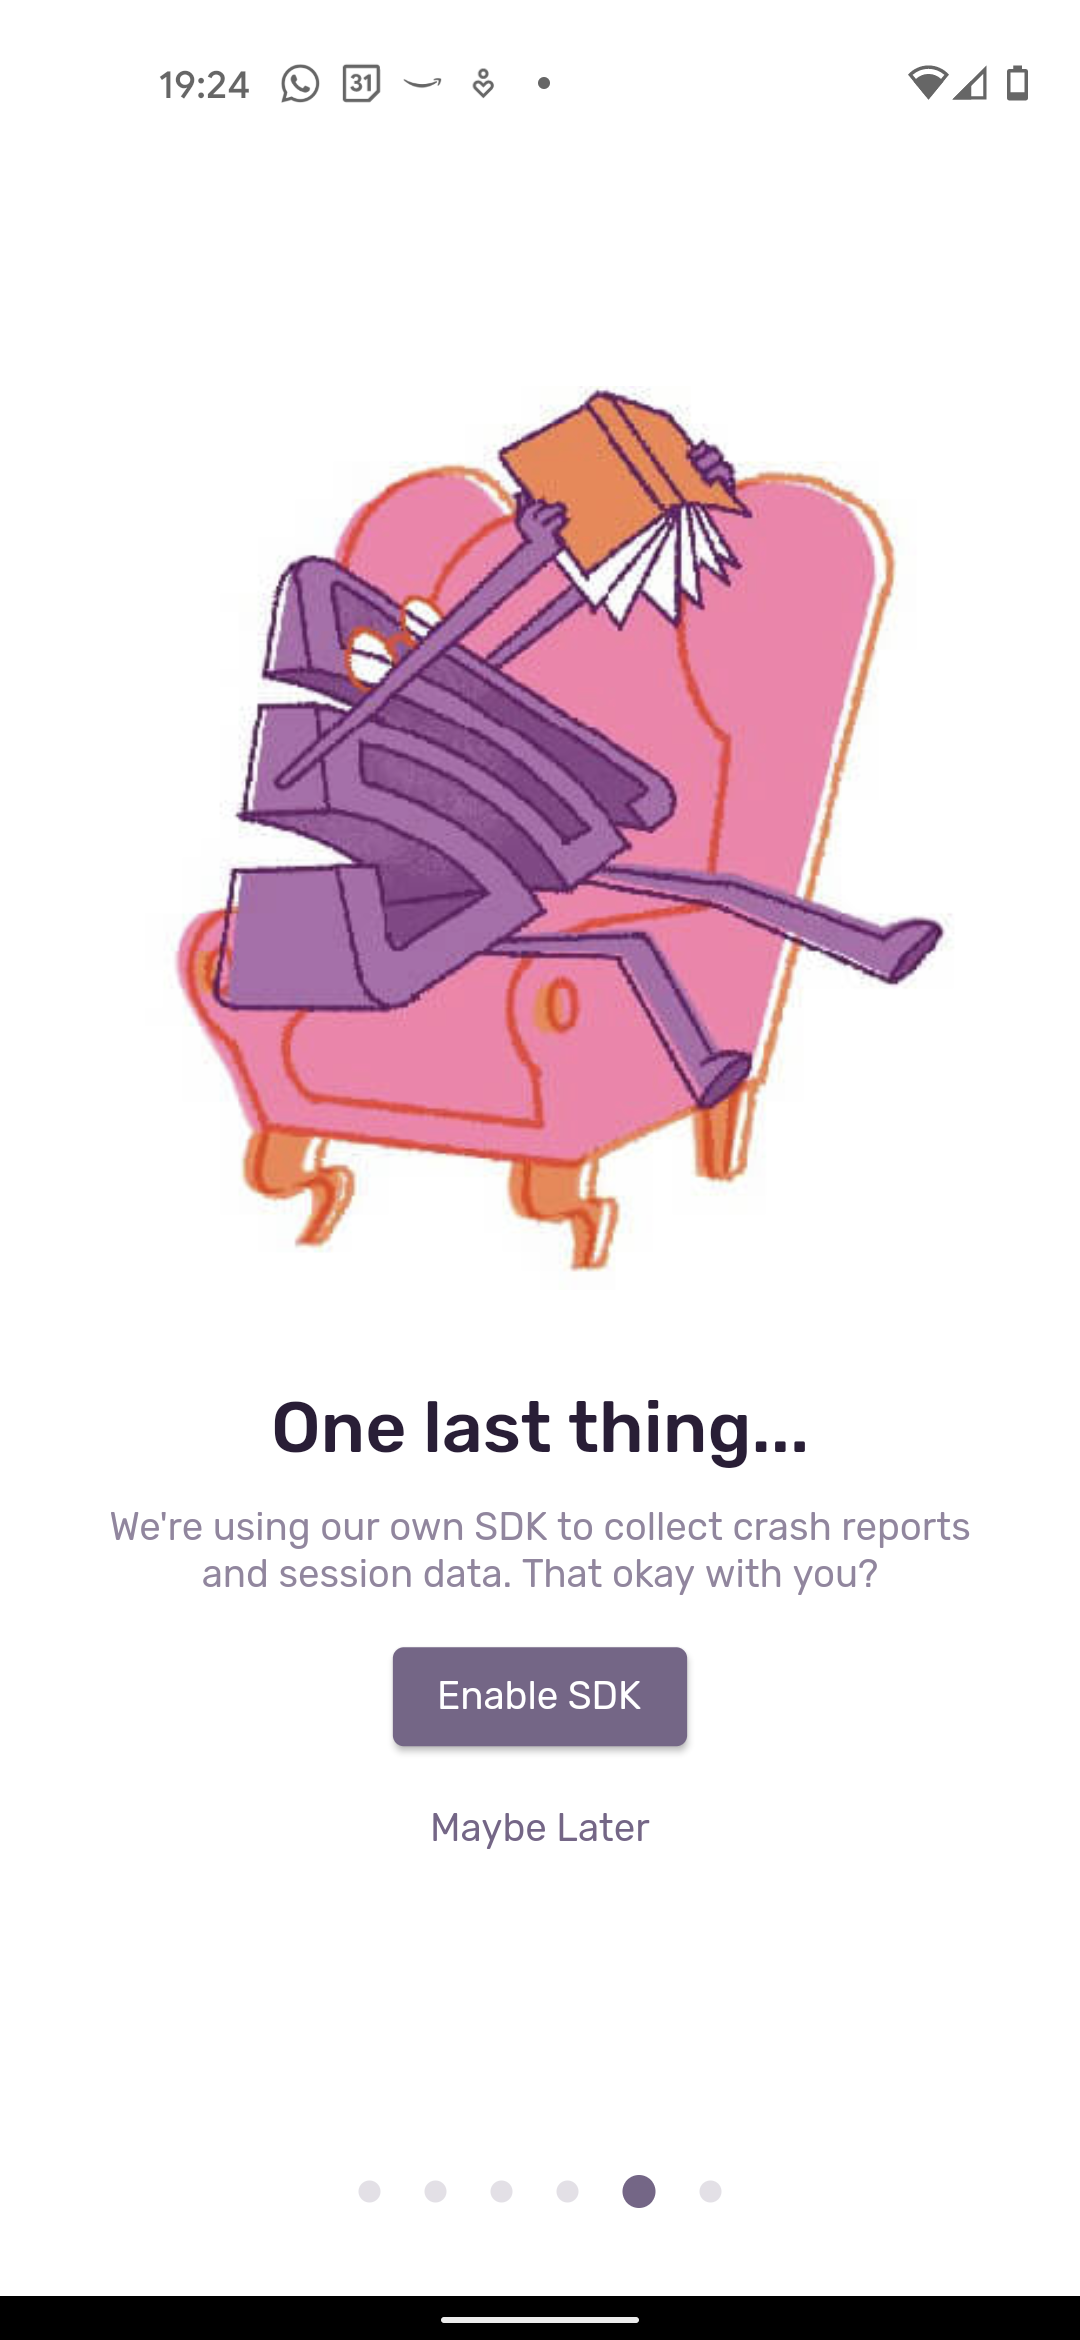
\includegraphics[width=5cm]{images/sentry.io/Screenshot_20210914-192435.png}
    \caption{sentry.io Android app uses their Analytics SDK}
    \label{fig:sentry-io-analytics-sdk-opt-in}
\end{figure}

\begin{figure}
    \centering
    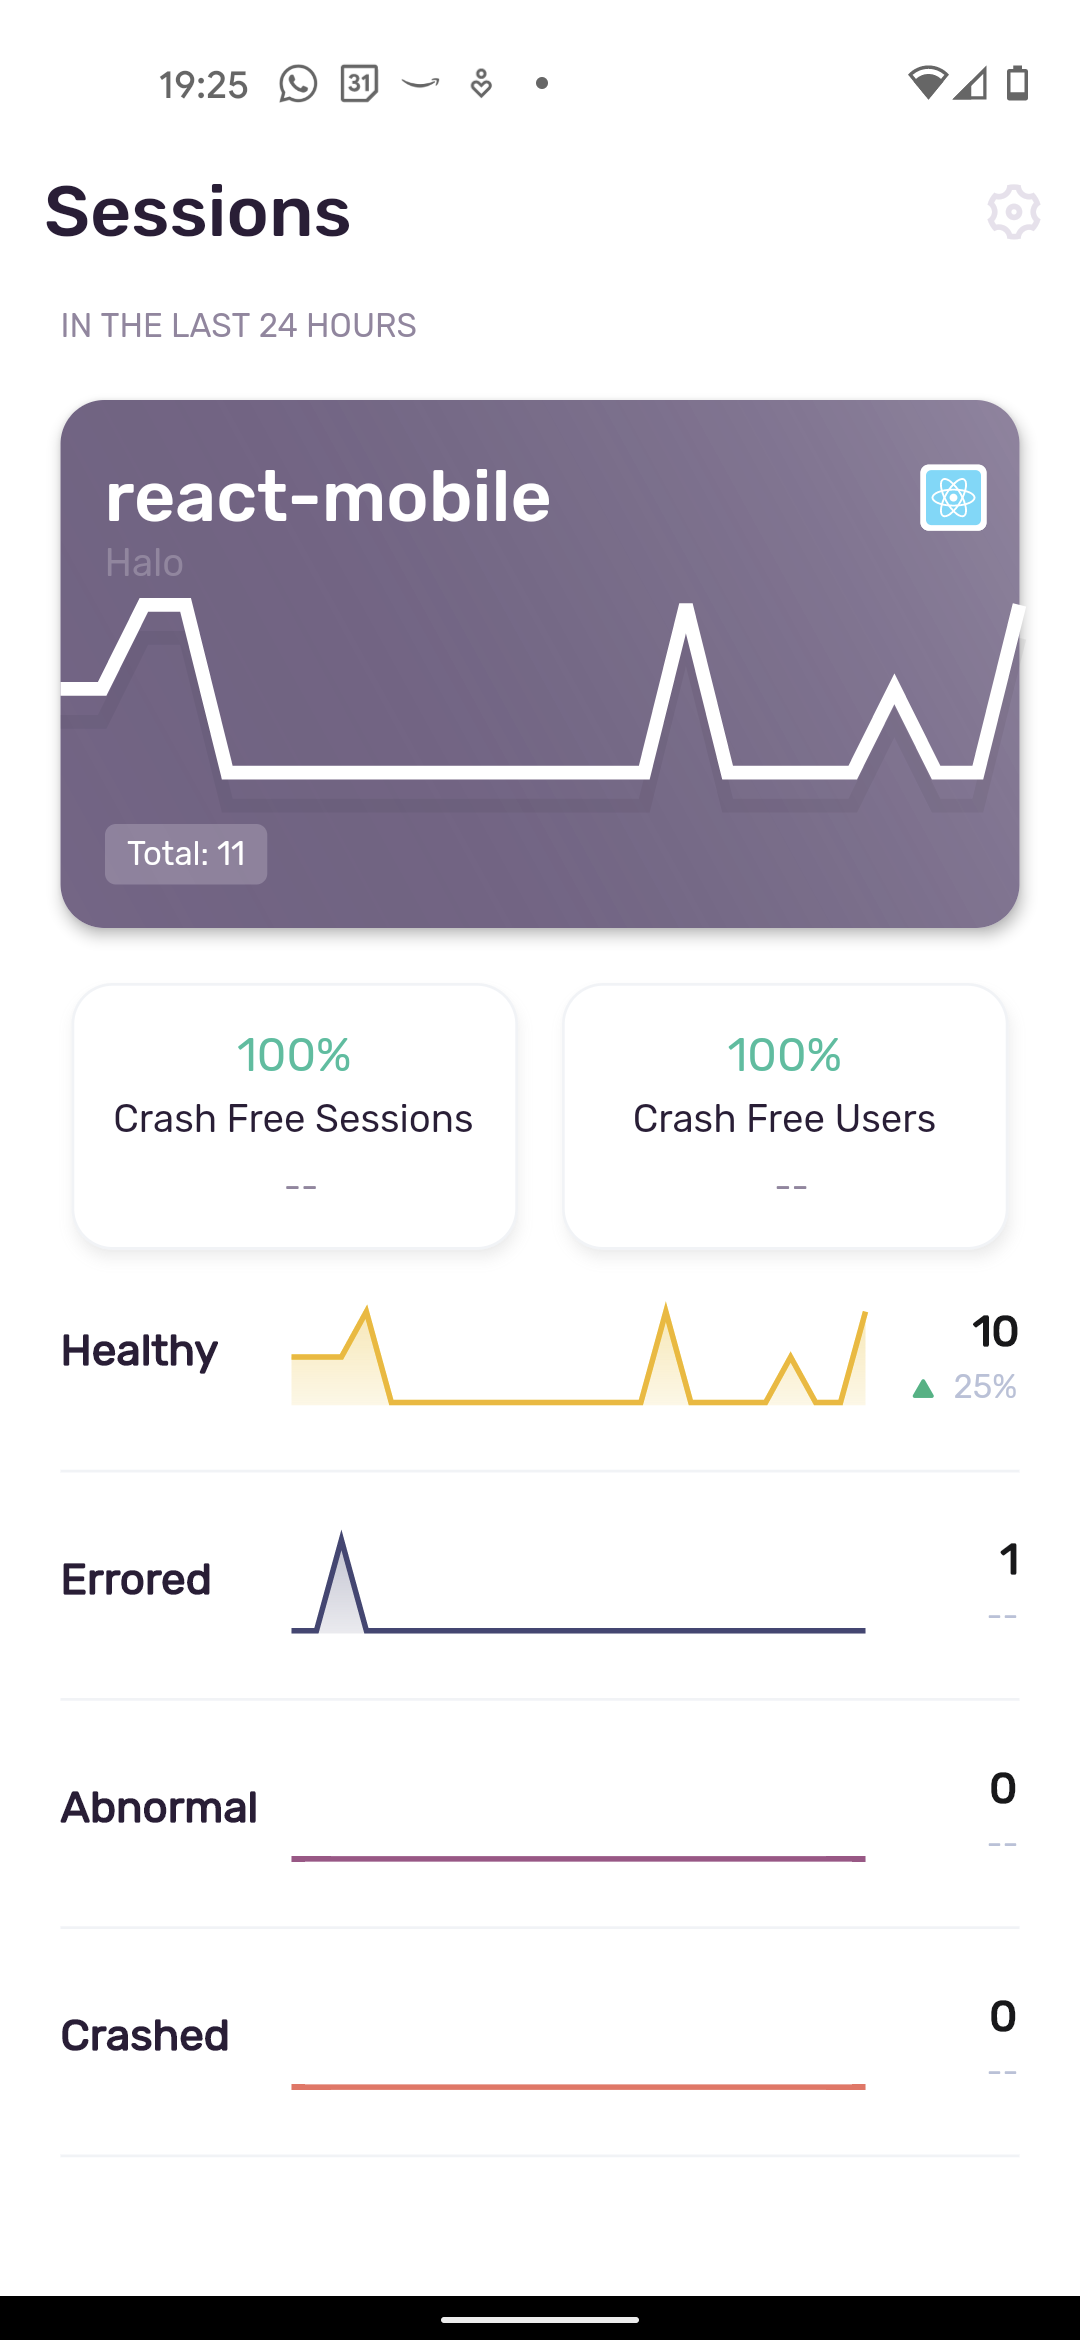
\includegraphics[width=5cm]{images/sentry.io/Screenshot_20210914-192538.png}
    \caption{sentry.io homescreen showing Release Health for the localhalo Android app}
    \label{fig:sentry-io-homescreen-release-health-for-localhalo-android}
\end{figure}


Sentry Developer plan 

\begin{itemize}
    \item Some useful pointers to topics of interest are fairly found in their busy twitter stream \url{https://twitter.com/getsentry}
    \item \emph{``See Slow Faster - Introducing Mobile Vitals"} on YouTube 53 minutes \url{https://www.youtube.com/watch?v=J0tAK6dKY3Y}
    \item Some vignettes in their customer story for ChartHop \url{https://sentry.io/customers/charthop/}
    \item On their hackathon that led to their early release mobile app \emph{``Sentry's New Mobile App for Managing Releases"}  \url{https://blog.sentry.io/2021/08/03/fluttering-our-mobile-wings}
    \item Customising dashboards \url{https://docs.sentry.io/product/dashboards/custom-dashboards/}
\end{itemize}

\section{Summary of Analytics Tools used in this research}
